\documentclass{beamer}
\usepackage[orientation=landscape,size=custom,width=106,height=90,scale=1.4,debug]{beamerposter}
\mode<presentation>{\usetheme{DVB}}
\usepackage[utf8]{inputenc}
\usepackage{hyperref} %enable hyperlink for urls
\usepackage{ragged2e}
\usepackage[font=scriptsize,justification=justified]{caption}
\usepackage{array,booktabs,tabularx}


\newcolumntype{Z}{>{\centering\arraybackslash}X} % centered tabularx columns

\title{\huge Born in a BARN: Bayesian Additive Regression Networks}
\author{Danielle Van Boxel$^{1}$}
\institute[UA:AM]{$^{1}$University of Arizona, Applied Math Program \\ \hphantom{1cm}}
\date{December 8, 2022}
\webpage{\href{github.com/dvbuntu/barn}{github.com/dvbuntu/barn} \raisebox{-.2\height}{\includegraphics[scale=0.4]{qr_barn}}}
\email{vanboxel@math.arizona.edu}
\posterlogo{gidp_am.png}

% edit this depending on how tall your header is. We should make this scaling automatic :-/
\newlength{\columnheight}
\setlength{\columnheight}{90cm}

\begin{document}
\begin{frame}
\begin{columns}
%%% BEGIN COLUMN 1
	\begin{column}{.33\textwidth}
	%\begin{beamercolorbox}[center]{postercolumn}
		\begin{minipage}{.98\textwidth}  % tweaks the width, makes a new \textwidth
		\parbox[t][\columnheight]{\textwidth}{ % must be some better way to set the the height, width and textwidth simultaneously
		\begin{myblock}{Brief Abstract}
%    We apply Bayesian Additive Regression Tree (BART) principles to training an ensemble of small neural networks for regression tasks.  Using Markov Chain Monte Carlo, Bayesian Additive Regression Networks (BARN) samples from the space of single hidden layer neural networks that are conditioned on their fit to data.  To create an ensemble of these, we apply Gibbs' sampling to update each network against the residual target value (i.e. subtracting the effect of the other networks).  We examine the effectiveness of BARN on several benchmark regression tasks, comparing it to equivalent neuron count single neural networks as well as equivalent tree count BART.  We also apply BARN to a more recent modeling problem and compare with state of the art.  BARN provides more consistent and often more accurate results, at the cost of significantly greater computation time.  BARN seems to perform best on problems with modest data and significant nonlinearity, though this needs further study.  It is highly adaptable, performing well on a variety of problems.
We adapt Bayesian Additive Regression Tree (BART)\cite{chipman2010bart} principles to training an ensemble of small neural networks\cite{schmidhuber2015deep} for regression tasks.  Using Markov Chain Monte Carlo\cite{hastings1970monte}, Bayesian Additive Regression Networks (BARN) samples from the space of single hidden layer neural networks that are conditioned on their fit to data.  BARN provides more consistent and often more accurate results, at the cost of significantly greater computation time.
		\end{myblock}
		\begin{myblock}{Background: Random Forests, BART, \& Beyond}
            \raggedleft{\Large{Random Forest}} \\ \vspace{-2em}
\begin{figure}[h]
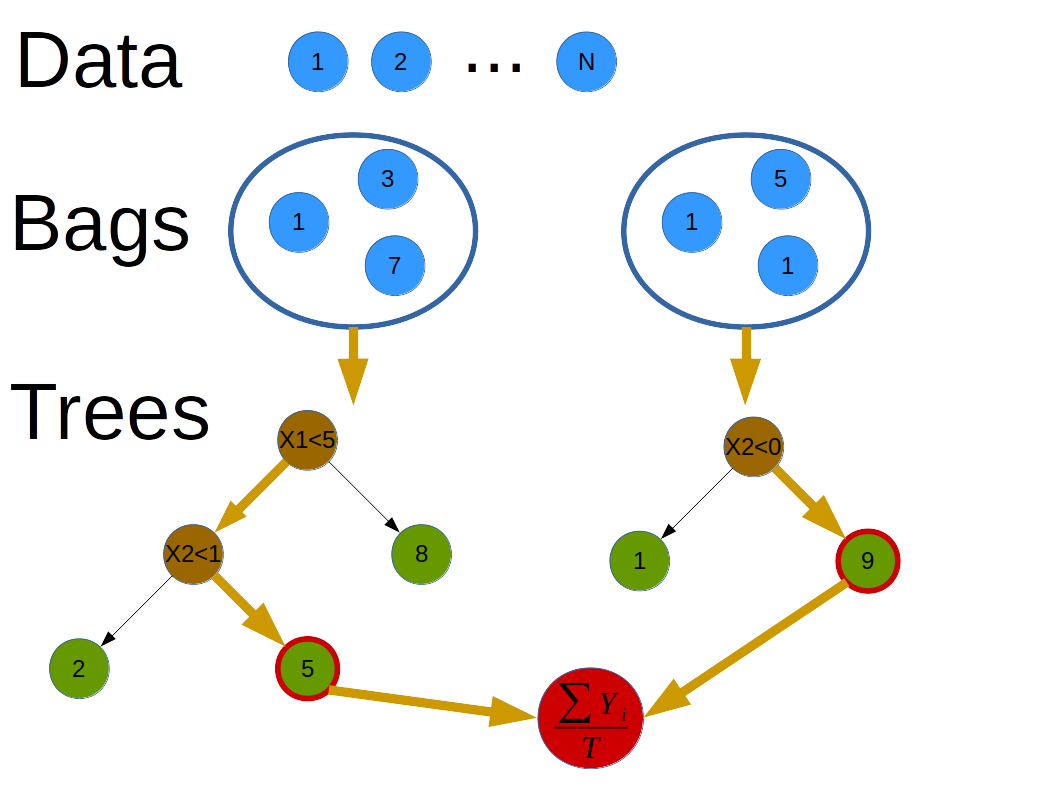
\includegraphics[scale=0.8]{pres_rf.png}
    \caption{Random Forest is ensemble of decision trees trained on different subdata sets \cite{breiman2001random}}
\end{figure}

            \raggedleft{\Large{BART}} \\ \vspace{-2em}
\begin{figure}[h]
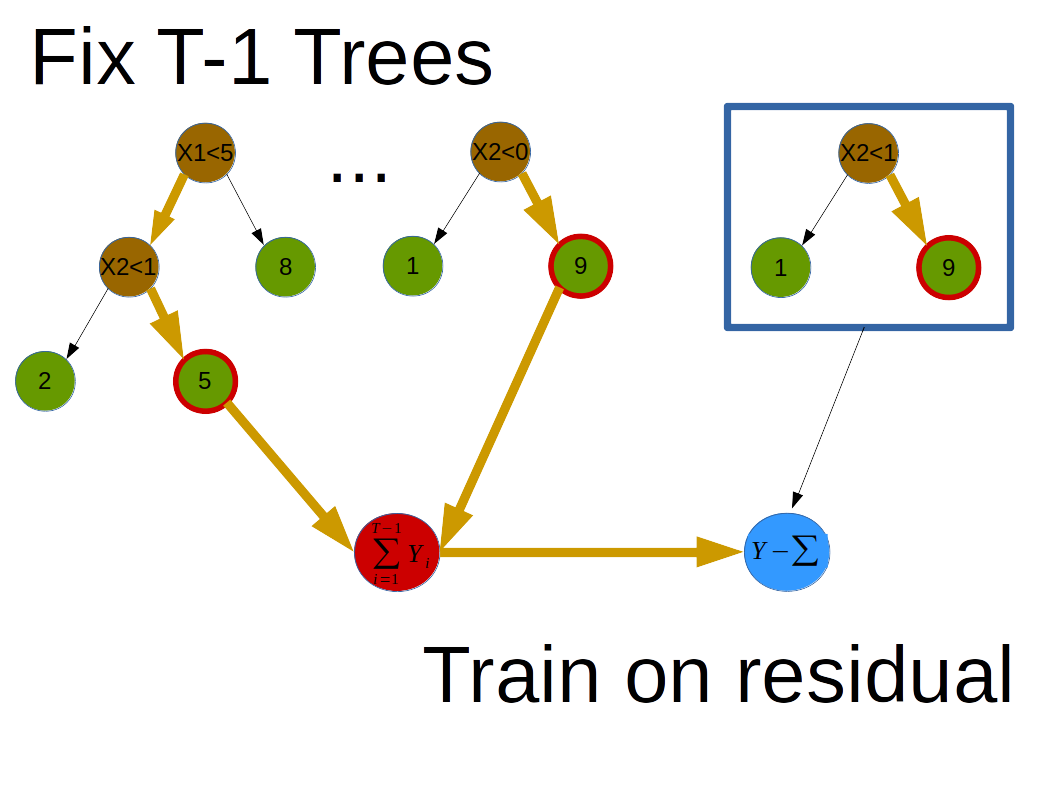
\includegraphics[scale=0.8]{pres_bart.png}
\caption{BART uses MCMC to sample from posterior of accurate reasonably sized decision trees by fixing all but one tree and proposing a small mutation \cite{chipman2010bart}}
\end{figure}

            \raggedleft{\Large{MCMC}} \\ \vspace{-1.5em}
\begin{figure}[h]
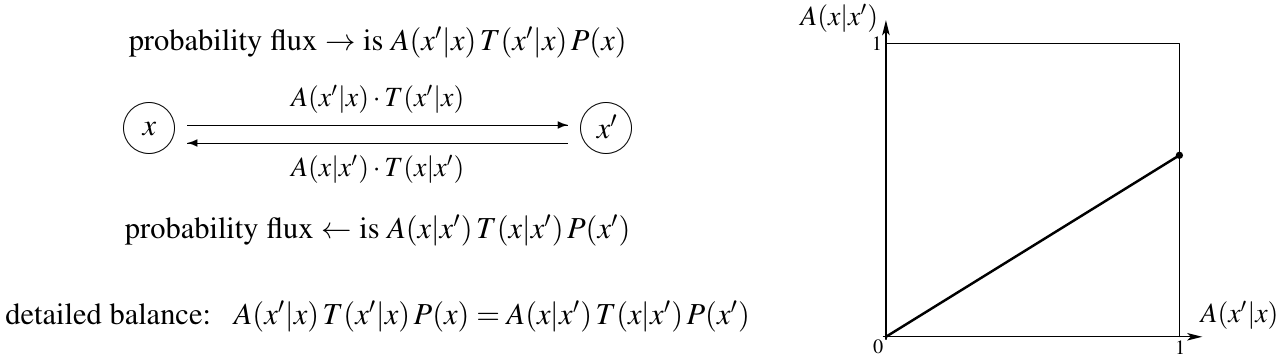
\includegraphics{balance.png}
\caption{Markov Chain Monte Carlo uses Accept/Reject to Maintain Stationary Distribution\cite{stepanov2021math}}
\end{figure}

            \raggedleft{\Large{NN Proposal}} \\ \vspace{-1.5em}
\begin{figure}[h]
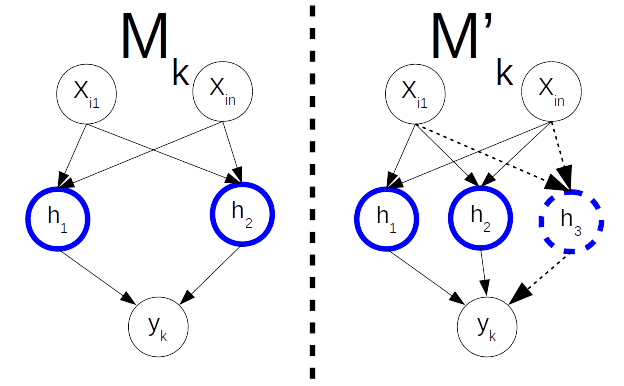
\includegraphics{barn_trans.png}
    \caption{Proposed mutation of neural network for BARN process adds or subtracts a neuron and retains weights}
\end{figure}
		\end{myblock}
	}
	\end{minipage}
	%\end{minipage}\end{beamercolorbox}
	\end{column}
%%% BEGIN COLUMN 2
	\begin{column}{.33\textwidth}
	%\begin{beamercolorbox}[center]{postercolumn}
	\begin{minipage}{.98\textwidth}  % tweaks the width, makes a new \textwidth
		\parbox[t][\columnheight]{\textwidth}{ % must be some better way to set the the height, width and textwidth simultaneously
			\begin{myblock}{BARN Fundamentals}

\begin{enumerate}
\item Initialize all networks to $M=1$ neuron
\item Gibbs' sample to propose one NN with residual
\item Train proposed $M_k'$, compute $A(M_k,M_k')$, Accept/reject
\item After burn-in period (default 100 steps), every step provides an ensemble of models, choose last/best (on validation)
\end{enumerate}

$$
\text{Acceptance: } A(M_k,M_k') = min(1, \frac{T(M_k|M_k') P(R_k|X,M_k')P(M_k')}{T(M_k'|M_k) P(R_k|X,M_k)P(M_k)})
$$

$$
\begin{aligned}
\text{Prior (Poisson): } & P(M) = \frac{\lambda^m e^{-\lambda}}{m!} \\
\text{Transition ($\pm1$ Node): } & T(M'|M) = \begin{cases}
			p & m' = m + 1 \\
			1-p & m' = m - 1 \\
\end{cases} \\
\text{Error (Normal Likelihood): } & P(R_k|X,M_k) \approx \prod_{i \in \text{valid}} \frac{e^{-\frac{1}{2}\left(\frac{(R_k-M_k(X_i))}{\sigma}\right)^2}}{\sigma \sqrt{2\pi}} \\
\end{aligned}
$$
			\end{myblock}
			\begin{myblock}{BARN Toy Example}
Starting with say $N=3$ networks in the ensemble and one validation data point, step through one iteration of fixing $M_1$ and $M_2$ while considering a new $M_3'$.

\begin{figure}[h]
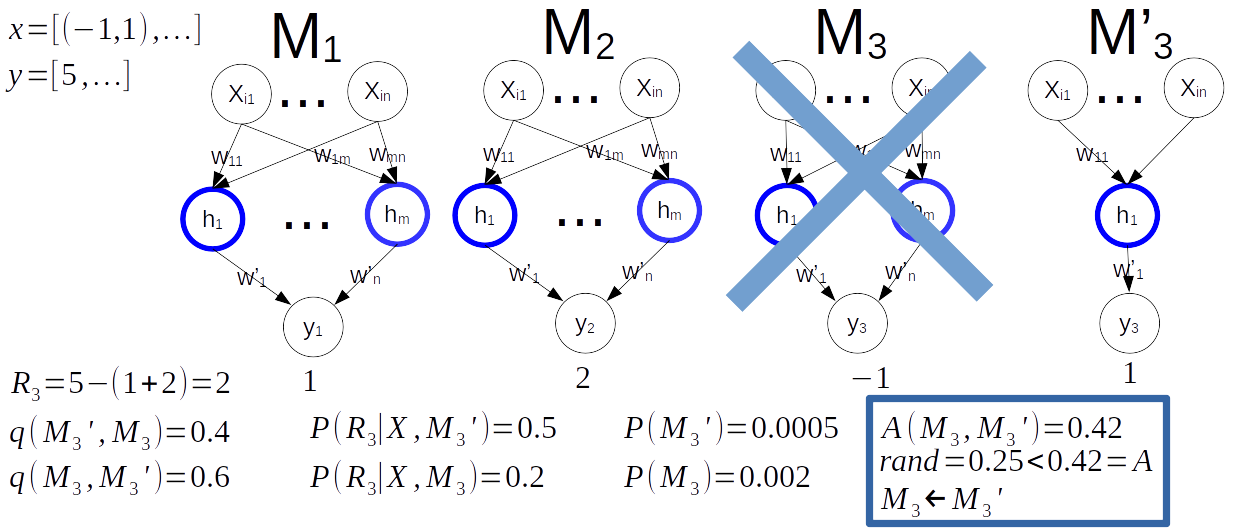
\includegraphics[scale=0.75]{barn_ex3.png}
    \caption{Fix $M_{i\neq 3}$, Propose and Train $M_3'$, Compute $A(M_3'|M_3)$, Accept $M_3'$}
\end{figure}
			\end{myblock}

		\begin{myblock}{BARN Benchmark Results}
\begin{figure}[h]
\centering
    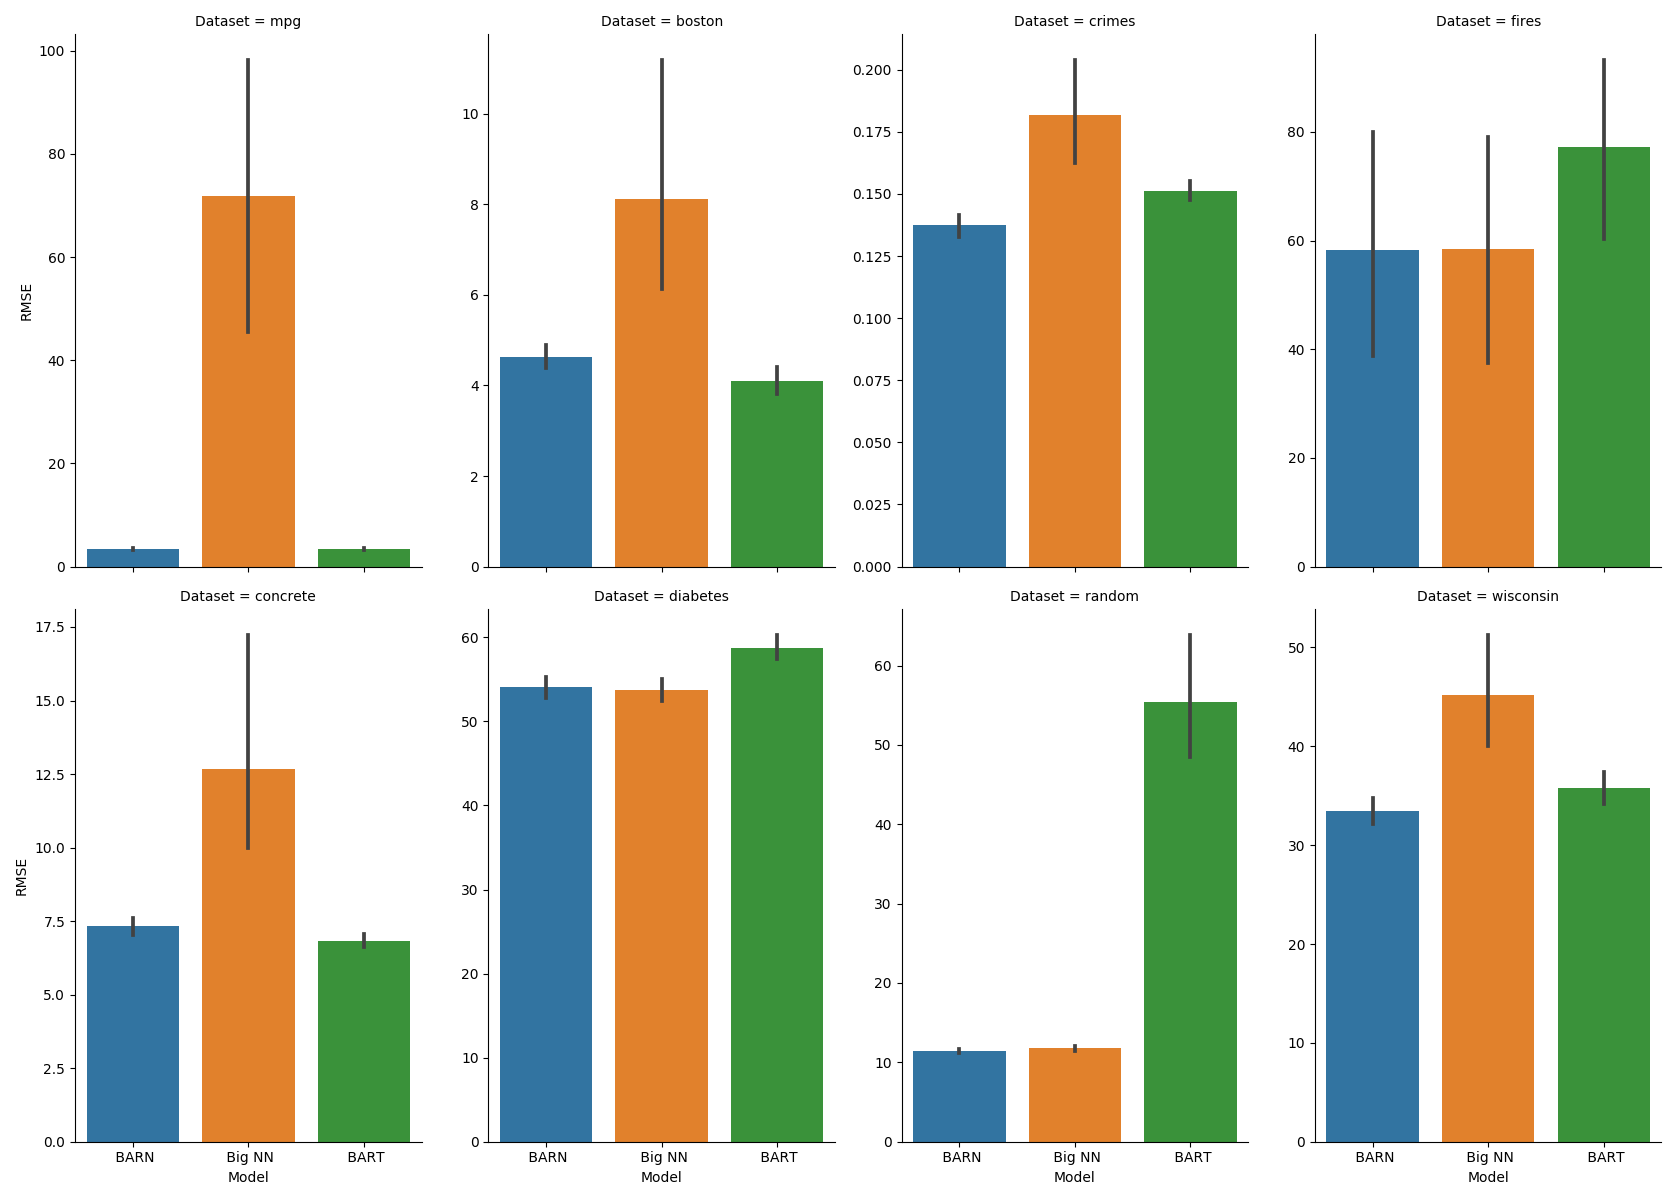
\includegraphics[scale=.62]{pres_results.png}
    \caption{BARN almost always matches or beats RMSE of other methods and is more stable}
    \label{fig:results}
\end{figure}

        \end{myblock}

	}

	\end{minipage}
	%\end{minipage}\end{beamercolorbox}
	\end{column}
%%% BEGIN COLUMN 3
	\begin{column}{.33\textwidth}
	\begin{minipage}{.98\textwidth}  % tweaks the width, makes a new \textwidth
		\parbox[t][\columnheight]{\textwidth}{ % pushes things to top
		\begin{myblock}{Additional BARN Results}
\begin{figure}[h]
\centering
    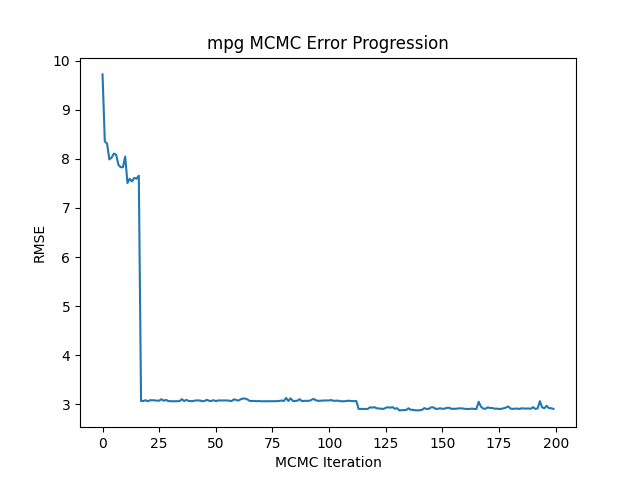
\includegraphics[scale=1.0]{mpg_phi.png}
    \caption{Typical error progression during BARN MCMC process shows convergence}
    \label{fig:error}
\end{figure}


\begin{figure}[h]
\centering
    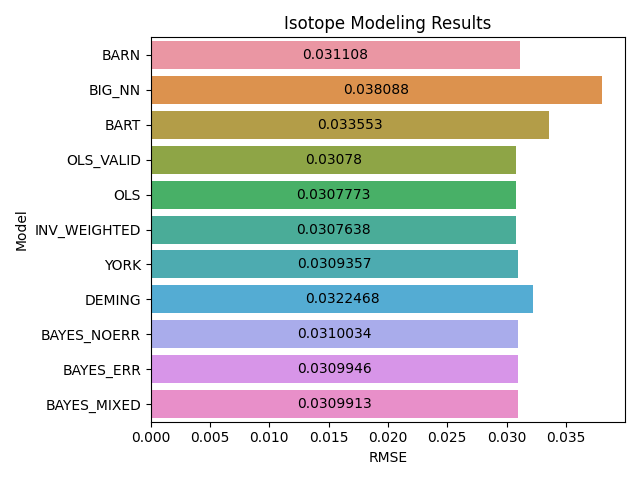
\includegraphics[scale=1.2]{iso_results.png}
    \caption{BARN can be competitive with state of the art results with minimal tuning}
    \label{fig:results_isotope}
\end{figure}

\begin{figure}[h]
\centering
    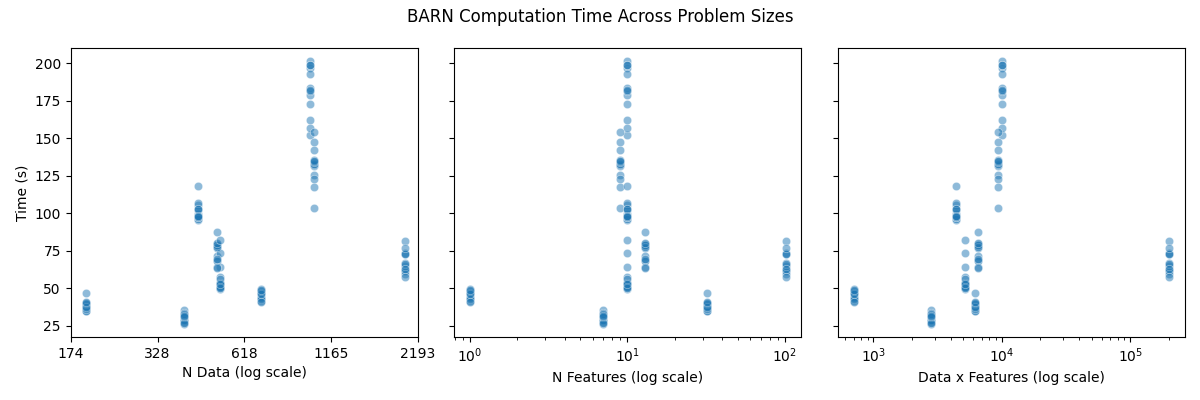
\includegraphics[scale=1.]{time_results.png}
    \caption{BARN may be slow even on small problems but time scales with difficulty, not just problem size}
    \label{fig:results_time}
\end{figure}

		\end{myblock}
			\begin{myblock}{Conclusion}
\begin{itemize}
\item Combines bayesian ensembling and architecture search
\item Error often minimal, but near other methods (i.e. $\pm 2\sigma$)
\item Computation time much longer for ($\approx$100s vs $\approx$0.1s)
\end{itemize}
		\end{myblock}
			\begin{myblock}{Further Work}
\begin{itemize}
\item Implement as \texttt{R} and Python package
\item Better justify model prior/transition probabilities
\item Generalize to \emph{arbitrary} ensemble-style models (SVMs?)
\end{itemize}
		\end{myblock}
		\begin{myblock}{References}
			\footnotesize
			\bibliographystyle{plain}
			%\bibliographystyle{plainnat}
			\bibliography{lib}
		\end{myblock}
		\vfill
		}
	\end{minipage}
	\end{column}
\end{columns}
\end{frame}
\end{document}
